\section{Evaluation}
\label{sec:evaluation}

\srm{Can we compare to some kind of ``baseline'' -- i.e., how well would these statistical methods do without access to expanded data?}

We implemented \dBoost/ as a library that runs on top of a standard relational database or set of structured data files. Our code is publicly available on GitHub under version 3 of the GNU Public License\footnote{\url{https://github.com/cpitclaudel/dBoost}}. The program is made of two parts: a library, and a number of data acquisition front-ends (CSV and SQL are currently supported). The library provides functions for each of the phases previously described, and includes a collection of generally useful expansion rules.

%Table~\ref{table:flags} shows the usage options to run the models supported by \dBoost/. \fxnote{Should we keep this table? ** Add an appendix if we have room}

%\begin{table*}
%  \renewcommand{\arraystretch}{1.2}
%  \setlength\tabcolsep{3\tabcolsep}
%
%  \label{table:flags}
%  \caption{\dBoost/ command line usage.}
%  \centering
%  \begin{tabular} { l | l | p{10cm} }
%    \multicolumn{3}{l}{} \\
%    \hline
%    Flag & Options & Explanation \\
%    \hline
%    --gaussian & n\_stdev & Report outliers that fall more than n\_stdev standard deviations away from the mean of the data \\
%    --mixture & n\_subpops & Use a model of \texttt{n\_subpops} Gaussians \\
%         & threshold & Report outliers above threshold percentile \\
%    --histogram & peak\_s & Consider only fields with a peaked distribution with peakiness peak\_s \\
%         & outlier\_s & Report values that fall in classes with less than outlier\_s percent \\
%    --statistical & epsilon & Give hints to the model for correlations with Pearson $R$ coefficient greater than epsilon \\
%  \end{tabular}
%\end{table*}

This section presents the results of running our tool on the following real and synthetic datasets.

\begin{itemize}
\item \emph{Synthetic datasets}\\
  \textbf{Fizz-Buzz} A mixed textual-numerical dataset in which each record contains two entries: a number, and either ``Fizz'' if the number is divisible by 3, ``Buzz'' if the number is divisible by 5, ``FizzBuzz'' if it is divisible by both, and the number itself (as a string) otherwise. Outliers appear when the second column does not respect these rules; this can be a misplaced ``Fizz'', a missing ``Buzz'', or even a totally different string (e.g. ``Woof!'').\\
  \textbf{Web logins} A series of three non-numeric datasets in which entries contain the login time and connection location for different users. Each user has different connection habits, leading to different types of outliers.
\item \emph{Real-world datasets}\\
  \textbf{CSAIL Directory} A publicly-accessible directory of researchers\fxnote{Should we anonymize this?}, in which each record may include a first and a last name, a phone number, an office number, an email, and a job title. Outliers are hard to define mathematically in this case, and we instead demonstrate how the ideas exposed in previous sections of the paper come together to allow for efficient detection of unusual values.\\
  \textbf{Intel lab data} A publicly-available numerical dataset of temperature, light, humidity and voltage measurements. Outliers are due mostly to sensor glitches.
\end{itemize}

These datasets showcase the power of our methods, both in terms of classification power and expressiveness and succinctness when adding new rules to the system\footnote{Indeed, the set of rules used for tuple expansion is user-configurable, and new rules can be easily added; thus, specific knowledge about the data can be taught to the system by users, expressing some soft form of data integrity constraints.}. Where relevant we include performance measurements. These numbers intend to demonstrate that our approach is computationally reasonable and that our models scale linearly given a fixed training size. We show in Section~\ref{sec:performance-evaluation} how our prototype requires on the order of a few minutes to process a million elements using a high-level single-threaded scripting language. A production-ready implementation would run one or two orders of magnitude faster by taking advantage of the inherent parallelizability of the models, using an efficient on-disk representation of the data, and relying on a lower-level language with an efficient optimizing compiler.

The following subsections describe each of the test sets and associated results in greater detail.

\subsection{Soft constraint specifications: Fizz-Buzz}
The Fizz-Buzz programming exercise is based on a children's game and frequently found in programming interviews. The synthetic dataset we generated obeys the following rules: for each record \texttt{<x, y>}, $x$ is a number between 0 and 1000, and $y$ is ``Fizz'' if \(x \mod 3 = 0\), ``Buzz'' if \(x \mod 5 = 0\), ``FizzBuzz'' if \(x \mod 15 == 0\), and \(x\) otherwise. However, we introduced three outliers to this data: \texttt{(25, "Fizz")}, \texttt{(28, "Woof!")}, \texttt{(30, "Buzz")}. Each demonstrates a different error, namely swapping \texttt{"Fizz"} and \texttt{"Buzz"}, producing entirely incorrect output, and failing to recognize that a number is divisible by both $3$ and $5$.

A traditional way of checking that all tuples verify the production rule outlined above is to encode this rule itself as a database integrity constraint. This requires encoding the full complexity of the exercise in the rule. If the exercise were to change, new cases must be added manually. Instead, a user might want to specify the bare minimum for the system to infer the rules; in this case, it is sufficient to add one extraction rule, mapping integers to two booleans denoting whether they are divisible by $3$ or $5$. Such a rule could be written like this:

\begin{minted}{python3}
@rule
def fizzbuzz(x: int) -> ("div 3", "div 5"):
  return (x % 3 == 0, x % 5 == 0)
\end{minted}

Running the discrete statistical analyzer on the synthetic datasets suggests that the two columns are correlated, and using the histogram model flags the aforementioned outliers. The output of the program for the \texttt{(30, "Buzz")} line, for example, is similar to:

\begin{lstnobreak}[gobble=2]
   $30$ $Buzz$
   > Values ($30$, $'Buzz'$) (0, 1) do not match
     features ($'div 3'$, $'erase numbers'$)
     • histogram for ('div 3', 'erase numbers'):
       █████ (False, 'Buzz')
       (False, 'Fizz')
       (False, 'Woof!')
       ██████████████████ (False, '<num>')
       $(True, 'Buzz')$
       ██████████ (True, 'Fizz')
       ██ (True, 'FizzBuzz')
\end{lstnobreak}

Using the partitioned histogram model produces similar output:

\begin{lstnobreak}[gobble=2]
   $30$ $Buzz$
   > Values ($30$, $'Buzz'$) (0, 1) do not match
     features ($'div 3'$, $'strp'$)
     • histogram for ('strp',) if 'div 3' = True:
       $('Buzz',)$
       ████████████████████ ('Fizz',)
       ████ ('FizzBuzz',)
     ... if 'div 3' = False:
       ████████████████████ ('<num>',)
       █████ ('Buzz',)
       ('Fizz',)
       ('Woof!',)
\end{lstnobreak}

\subsection{Logins: a more realistic partitioned dataset}

Our web activity synthetic datasets are comprised of two columns: a Unix timestamp stored as an \texttt{INT}, and a country. Each dataset is supposed to track the connections of a registered user on a website; such a dataset could be obtained by selecting the relevant rows out of a large table listing all connections of all users. Each user exhibits a different connection pattern:

\begin{itemize}
\item One user always connects from the same country; values that do not match this country are outliers.
\item The second connects from one country during the week, and from another during the week-end; outliers in this case are connections from a country that doesn't match the country for that day of the week.
\item The third user connects from a set of three countries, with no discernible pattern. This should not return any outliers.
\end{itemize}

The datasets are randomly generated sets of 2000 connections, listed in no particular order. The target outlier rate is \SI{5}{\percent} in each generated dataset.

\newcommand{\prop}[2]{#1\,\#\,#2}

Just like in the \emph{Fizz-Buzz} example, numerical models are useless here, and histogram-based models fare well. In the first case, a histogram-based model with no correlation analysis is sufficient to flag the outliers. In the second case, the discrete statistical analysis phase singles out interesting pairs of correlated columns, including \texttt{(\prop{date}{day of week}, country)} and \texttt{(\prop{date}{is weekend}, country)}. A histogram-based model is sufficient to successfully flag outliers, without resorting to partitioning.

\fxnote{Exclude self-correlations from the discrete analyzer to speed it up and get better results}

Mixing data from two or more users, however, shows the limits of the non-partitioned histogram approach. If we only look at two-columns correlations the individual behavior patterns become less apparent, and if we look at three-column correlations the histograms become too large and spurious hits start to appear due to the many discrete correlations hints returned by the analyzer. The partitioned histograms model, on the other hand, can handle the three-users without particular difficulties, by highlighting (among others) the triplet \texttt{(user, \prop{date}{is weekend}, country)}

\subsection{CSAIL Directory}
\label{sec:csail-directory-evaluation}

The CSAIL directory is an online directory of about 1000 faculty, staff and students in the MIT Computer Science and Artificial Intelligence Laboratory\footnote{\url{https://www.csail.mit.edu/peoplesearch}}. Each entry contains a person's name, phone number, office number, email address, and position.

Some data, such as a phone number, may be missing from the directory. Still, we expect our framework to be useful in flagging discrepancies between different records. Since the notion of what constitutes an outlier here is imprecise at best, we also expect the tool to allow the user to explore different sets of parameters. To illustrate the process, we present the results returned by two iterations of the tool in the next subsection, each with increasingly strict limits on the number of outliers returned. Because the CSAIL test set is exclusively textual, we use the histogram model for evaluation; continuous models would not fare as well, since only part of the expanded tuples are numeric.

\subsubsection{Initial run: low specificity filtering}
The search for outliers is initiated with parameters $\theta = 0.8, \epsilon = 0.2$. Correlation detection is disabled for these experiments.

This invocation produces a long list of outliers; a small subset of these is presented below. For privacy reasons, names,  phone numbers, office numbers, and emails have been omitted or anonymized in the following listings.

\begin{lstlisting}[gobble=2]
  Hacker, Alyssa, 32-D968,
    $aph@CSAIL.MIT.EDU$, Postdoctoral Associate

  Bitdiddle, Ben, $NE47-989$,
    bbitdid@mit.edu, Graduate Student

  $Lu-ater$, Eva, 32-G972,
    eva@csail.mit.edu, Research Scientist

  Tweakit, $ $, 32-G699,
    twktem@mit.edu, Administrative Assistant
\end{lstlisting}

In total, 451 entries contain outliers, out of a total of 1000. Office numbers are often flagged, as well as names and email addresses. By changing the input parameters to $\theta = 0.8, \epsilon = 0.05$, most of the outliers due to office numbers disappear due to the lower sensitivity. \lstinline{Hacker, Alyssa} disappears from the list, since e-mails with inconsistent capitalization occur frequently enough in the database that they are not considered outliers at sensitivity level $\epsilon = 0.05$. In total there are $68$ outliers.

\begin{lstlisting}[gobble=2]
  Bitdiddle, Ben, $NE47-989$,
    bbitdid@csail.mit.edu, Graduate Student
  > Value '$NE47-989$' doesn't match feature '$signature$'

  $Lu-ater$, Eva, 32-G972,
    eva@csail.mit.edu, Research Scientist
  > Value '$Lu-ater$' doesn't match feature '$title case$'

  Tweakit, $ $, 32-G699,
    twktem@mit.edu, Administrative Assistant ...
  > Value '$ $' doesn't match feature '$empty$'
\end{lstlisting}

In addition to identifying outliers, dBoost is equipped with tools that provide the user with additional feedback on why features were identified as outliers.

\begin{lstlisting}[gobble=2]
  Bitdiddle, Ben, $NE47-989$,
    bbitdid@csail.mit.edu, Graduate Student
   > Value '$NE47-223$' doesn't match feature '$signature$'
   • histogram for ('signature',):
     [266] ██████████ <empty>
     [  1] /▌/ $Lu,Lu,Nd,Nd,Pd,Nd,Nd,Nd$
     [  1] ▌ Lu,Nd,Nd,Pd,Nd,Nd,Nd
     [  2] ▌ Nd,Nd,Lu,Pd,Nd,Nd,Nd
     [485] ████████████████████ Nd,Nd,Pd,Lu,Nd,Nd,Nd
     [ 51] ██ Nd,Nd,Pd,Lu,Nd,Nd,Nd,Lu
     [155] ██████ Nd,Nd,Pd,Nd,Nd,Nd
     [ 36] █ Nd,Nd,Pd,Nd,Nd,Nd,Lu
     [  3] ▌ Nd,Nd,Pd,Nd,Nd,Nd,Nd
     [  1] ▌ Nd,Pd,Nd,Nd,Nd

  $Lu-ater$, Eva, 32-G972,
    eva@csail.mit.edu, Research Scientist
  > Value '$Lu-ater$' doesn't match feature '$title case$'
  • histogram for ('$title case$',):
    [ 15] /▌/ $False$
    [986] ████████████████████ True

  Tweakit, $ $, 32-G699,
    twktem@mit.edu, Administrative Assistant ...
  > Value '$ $' doesn't match feature '$empty$'
  • histogram for ('empty',):
    [1000] ████████████████████ False
    [   1] /▌/ $True$
\end{lstlisting}

Our tool highlights the incorrect field, and prints the corresponding histogram. The bin in which the suspicious value falls is also highlighted. The \texttt{signature} case is particularly interesting: recall that to extract the signature of a string, our tools replace each character by the name of its Unicode class; hence the string \texttt{NE47-989} is converted to \lstinline{Lu,Lu,Nd,Nd,Pd,Nd,Nd,Nd} (two letters, two numbers, one dash, three numbers), which does not fall in any of the dominant bins (the most frequent case, \lstinline{Nd,Nd,Pd,Lu,Nd,Nd,Nd}, describes office numbers like \lstinline{32-G804}, the predominant form of office numbering in the Stata Center).

Manual inspection of the results reveal that most of the outliers reported are actually bad inputs. There are, however, a number of false positives, such as:

\begin{lstlisting}[gobble=2]
  $DeFect$, Cy, 32-D597,
    cydf@csail.mit.edu, Graduate Student
  > Value '$DeFect$' doesn't match feature '$title case$'
  • histogram for ('$title case$',):
    [ 15] /▌/ $False$
    [986] ████████████████████ True
\end{lstlisting}

The case of \lstinline{DeFect} is correct, but our tool notes that it does not adhere to the casing standard derived from other tuples, and thus reports it.

\begin{figure*}
  \includegraphics{../graphics/csail-stats}
  \caption{Accuracy of dBoost on the CSAIL dataset -- Outliers were detected using a modality factor of 0.9 and a threshold of 0..075}
  \label{fig:csail-evaluation}
\end{figure*}
\subsection{Intel Lab Data}
\label{sec:intel-lab-data-evaluation}

We also evaluated our outlier detection framework on sensor data from the publicly available Intel Lab Data set~\footnote{\url{http://db.csail.mit.edu/labdata/labdata.html}}. The Intel Lab Data contains data collected from 54 sensors spread throughout the Intel Berkeley Research Lab. Each data entry contains information including humidity, temperature, light and voltage taken from a Micro2dot sensor and weatherboard. The dataset contains a total of approximately 2.3 million measurements.

The Intel lab dataset has known outliers from faulty sensor readings due to periods of critically low voltage. During these periods, the sensors go haywire and produce faulty measurements.

Due to the numerical nature of this data, the Simple Gaussian and Mixture models are well suited to analyzing it. However, the Histogram model does not fare as well.

% Random Sample 1000 data points
We analyzed a sample of 1000 data points selected at random from the data set. Figure~\ref{fig:sensors_1k_gm} shows the results from the simple Gaussian model comparing voltage and temperature; we set the tolerance ($\theta$) to 2. Since this model does not use correlation hints, the threshold for the statistical analyzer is irrelevant.

We observed that while this simple model is able to detect the high and low voltage outliers, it also identifies points within the main cluster of the data between 20 and 30 Celsius. These outliers are primarily due to light measurements whose measurements fall more than 2 standard deviations above the norm. When only outliers from temperature and voltage are taken into account, the outliers fall on the highest and lowest temperatures, as expected.

Figure~\ref{fig:sensors_1k_mm} shows the Mixture model results for the same 1000 randomly-selected data points. We used $0.75$ as the threshold $\theta$ to determine correlation, 3 Gaussians to populate our model, and returned $17\%$ of the data as outliers.

The statistical analyzer produces two correlations: one between temperature and voltage with an $R$ coefficient of $-0.75$ and between temperature and humidity with an $R$ of $-0.8$. The resulting Mixture models flags outliers that register temperatures of over 120 degrees. The outliers detected in the main cluster are the result of points that do not follow from the correlation between temperature and humidity.

\begin{figure}[h]
\centering
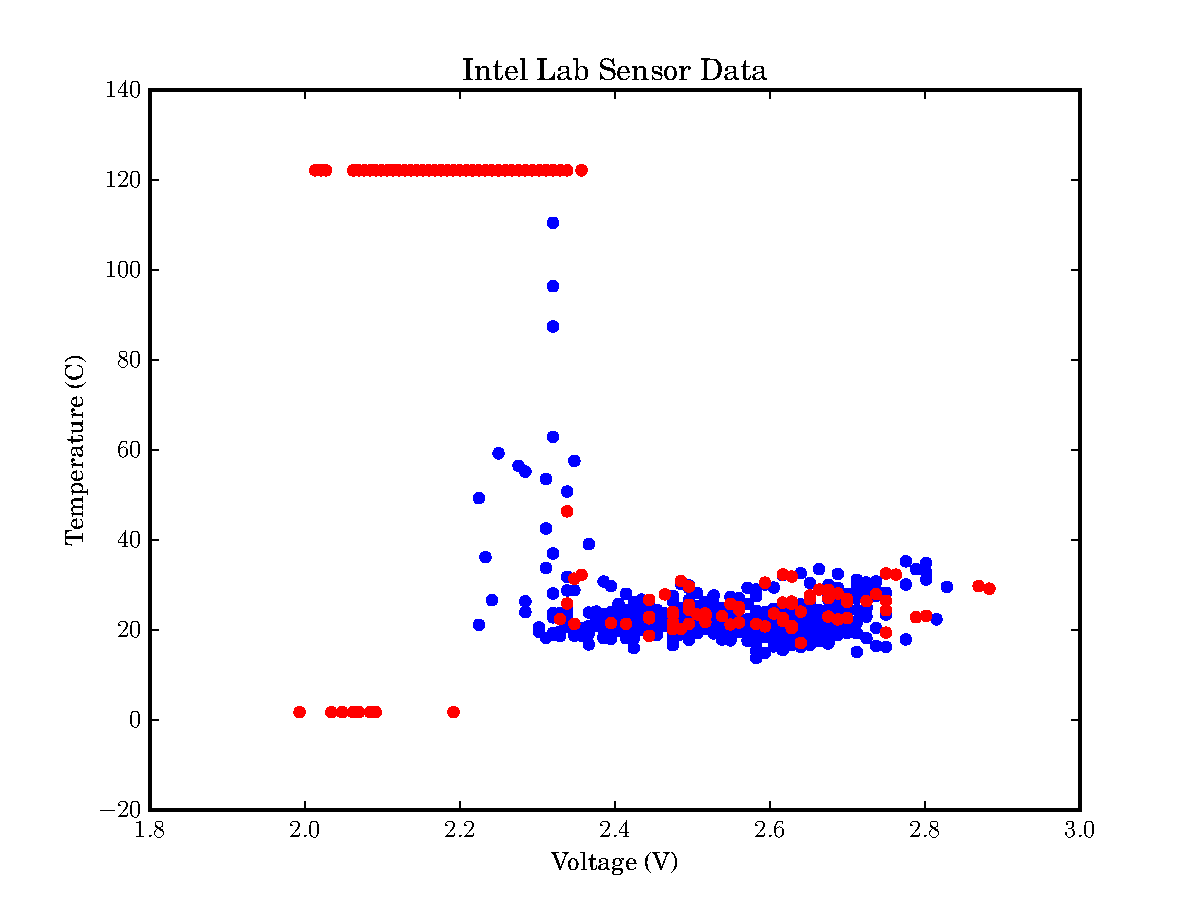
\includegraphics[width=0.45\textwidth]{../graphics/plots/sensors_gm.pdf}
\caption{Outliers from sensor data detected by a Gaussian model.}
\label{fig:sensors_1k_gm}
\end{figure}
\begin{figure}[h]
\centering
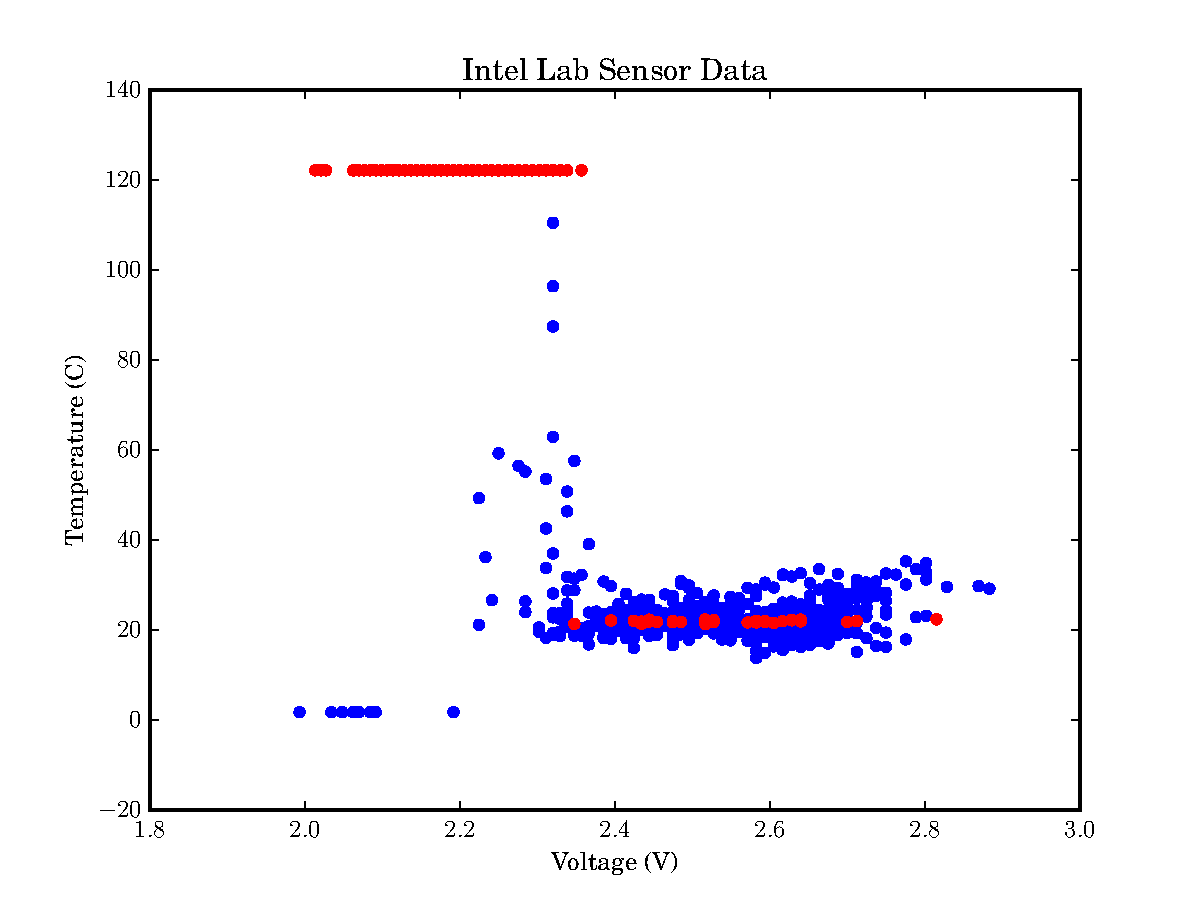
\includegraphics[width=0.45\textwidth]{../graphics/plots/sensors_mm.pdf}
\caption{Outliers from sensor data detected by a Mixture model.}
\label{fig:sensors_1k_mm}
\end{figure}

\subsection{Scalability}
\label{sec:performance-evaluation}

%We show in Figure~\ref{fig:scaling} how \dBoost/ scales as the amount of data used to build the models and to test on the models increases.
We measure the total runtime of our system, including the data modeling and outlier detection phases for the Simple Gaussian, Mixtures with 2 Gaussians, and Histograms. 
We used the Intel sensor data set from Section~\ref{sec:intel-lab-data-evaluation} to evaulate the Gaussian and Mixture models, and the CSAIL directory from Section~\ref{sec:csail-directory-evaluation} to evaluate the Histograms. 
We use random sampling to provide training sets of 1 thousand and 10 thousand elements from the Intel dataset to build the data models.
We test them on all 2+ million elements in the dataset.
To provide a more comprehensive study of the scalability of the Histogram model, we replicated the rows of the CSAIL directory to increase the training and test set sizes. 

In Figure~\ref{fig:scaling}, we show the runtime of our prototype. Each line shows a model trained with a different training set size. As shown in the figure, runtime scales linearly as the test set size increases.
Applying additional optimizations such as using a lower-level language or enabling parallism would improve runtime performance to production-ready levels. 

\begin{figure}
\centering
\paddedgraphics{../../graphics/scalability.pdf}
\caption{The scalability of the Gaussian and Mixture Models produced with different training sample sizes (listed next to the model in the legend) as the test set size increases.}
\label{fig:scaling}
\end{figure}

%\subsection{Presidential Campaign Finance}
\label{sec:presidential-campaign-evaluation}
\cite{PresCampaignData}

%\subsection{Mimic2}
\label{sec:mimic2-evaluation}

